\section{User Experiment}

We conducted an experiment to assess the validity of our system. The experiment has two parts.

Part A was to confirms the network delay requirement. We choose a task with high temporal synchronicity: the Rock-Paper-Scissor game. The experiment assesses users' perception of network delay in two conditions: with and without the sync assistance. 

Part B was to assess the user experience in the fully co-present situation. The task was the remote chess game that requires a high level of co-presence. We summarized result from observation and interview.

\subsection{Part A: Rock-Paper-Scissors}

\subsubsection{Experimental design}

This part was a within-subjects design. Each pair played the Rock-Paper-Scissors game in two sessions: with and without the sync assistance. We applied Latin square to the two sessions. In each session, we tested the one-way delay of 50, 83, 117 and 150ms in four trials in a random order. The network delay of our system is 50 ms. In the experiment, we added artificial delay if necessary.

\subsubsection{Task}

In each trial, a pair show the Rock-Paper-Scissors gestures for ten times. In the condition with sync assistance, the users show the gestures according to the sync assistance. In the condition without sync assistance, each participant was asked to start the game for five times, e.g., by saying "Three, two, one, go!". The reason for this requirement is that the delay perceptions of the starter and his partner are different \cite{hashimoto2006influences}.

\subsection{Part B: Playing Chess}

\subsubsection{Experimental design}

Each pair played chess remotely in five trials of three minutes. The one-way delay was 50 ms. The audio channel was open so that the users can chat in the game.

\subsubsection{Task}

In each trail, the two participants played chess "face-to-face" for three minutes. We adopted \emph{Reversi} as the task. The game is simple enough that the participants can learn it in two minutes. Each player owns an assigned color of chess pieces. Players take turn placing pieces on the chessboard. Any opponent' s pieces that are in a straight line and bounded by the piece just placed and another current player' s piece are captured. The captured pieces should be replaced by the current player' s pieces. In our system, the user can not actually touch the opponent' s pieces. He should ask the opponent to remove the captured pieces.

\subsection{Participants}

We advertised our experiment on social media. Sixteen pairs of participants took part in our experiment (32 in total, 7 females). They all came from the campus, aged from 18 to 24. Participants were paid 100 yuan for the 60 minutes long experiment.

Each pair of participants are familiar with each other (friends, classmates or partners). This is to improve the conversation quality. According to the self-report questionnaire, the participants are quite familiar with multimedia (3.50 points in average, 5 for experts) and AR/VR (2.89 points in average).

\subsection{Procedure}

Before the experiment, we invited the participant pair to a room and explained our study. We explained the rule of \emph{Reversi} and \emph{Rock-Paper-Scissors}. Next, the pair had ten minutes to experience the physical interaction of the two games. Then, we introduced our experimental procedure to the participants.

Part A had 2 sessions $\times$ 4 trials = 8 trials, which lasted for 20 minutes. Part B had one session of 5 trials (20 minutes). In each trial, the participants experience the game. After each trial, participants rested for one minute.

In the Rock-Paper-Scissors game, the network delay in each trip is different. We did not tell the participants the actual value of network delay. They filled in a short survey after each condition of network delay. The survey questions are on a 5-point likert scale (Table \ref{tab:table_experiment}):

\begin{table} [!htbp]
\begin{tabular}{|p{0.25\columnwidth}|p{0.35\columnwidth}|p{0.3\columnwidth}|}
\hline 
Label & Question & Scale (1 <--> 5) \\
\hline
noticeability & Can you perceive the network delay in the connection? & Very much <--> Not at all \\
\hline
network quality & How do you feel about the network quality? & Bad <--> Excellent \\
\hline
\end{tabular}
\caption{The questionnaire for each condition of network delay in the Rock-Paper-Scissors game. The users did not know the value of network delay.}
\label{tab:table_experiment}
\end{table}

Between the two tasks, participants had a five minutes break. After each task was a brief interview to investigate users' acceptance of rendering quality and network delay. The questions are as followed:

\begin{itemize}
    \item Can you accept the rendering quality (Yes/No)?
    
    \item Did the rendering quality affect the task (Yes/No)?

    \item Can you perceive the network delay? What are the cues?
    
    %\item What makes you annoyed in the task?
    
    \item Any other comments?
\end{itemize}

\subsection{Assessment of temporal synchronicity}

We analyze the result of the Rock-Paper-Scissors game to assess the temporal synchronicity. The independent variables are network delays and whether there is a sync assistance. The dependent variables are the noticeability of network delays and the overall rating of network quality.

\begin{figure}[!htbp]
\centering
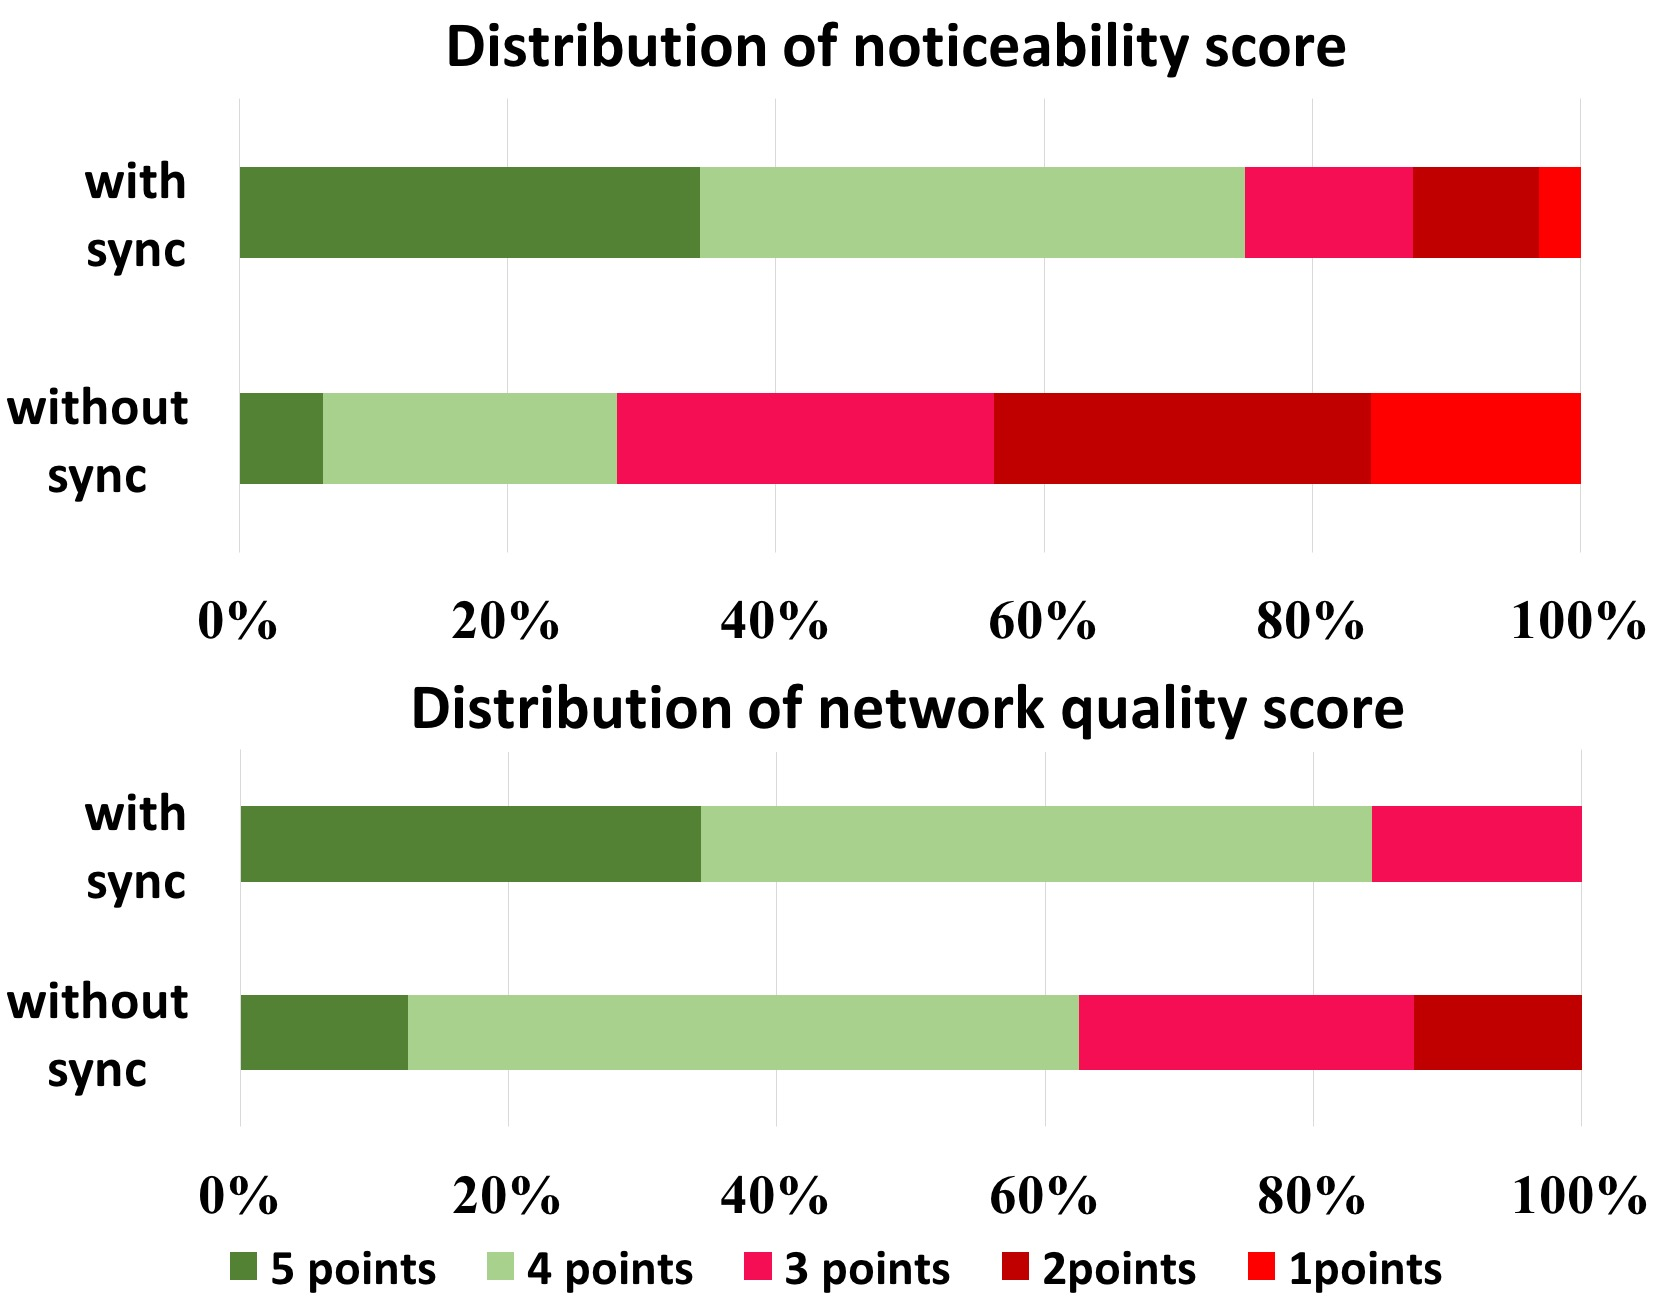
\includegraphics[width=0.98\linewidth]{figures/figure7_1.jpg}
\setlength{\abovecaptionskip}{0.5cm}
\caption{The upper figure shows the percentage of each subjective score for the noticeability. The lower figure is for the network quality.}
\label{fig:subjective_rating_50ms}
\end{figure}

We first evaluate the subjective feedback of our system synchronicity. Given that we used direct Ethernet connection, our network delay of 50 ms was the only factor to affect network quality \cite{donovan2014understanding}. As figure \ref{fig:subjective_rating_50ms} shows, the network delay of our system was noticeable for most users as the game requires a very high synchronicity. 3.5 MOS is a standard for good user experience in tele-communications \cite{enderes2002impact, schaefer2002subjective}. Without the sync assistance, 62.5\% participants scored more that 3.5 points to the network quality, while the percentage was 84.4\% with the sync assistance. It shows that synchronicity of our system is acceptable for most users.

\begin{figure}[!htbp]
\centering
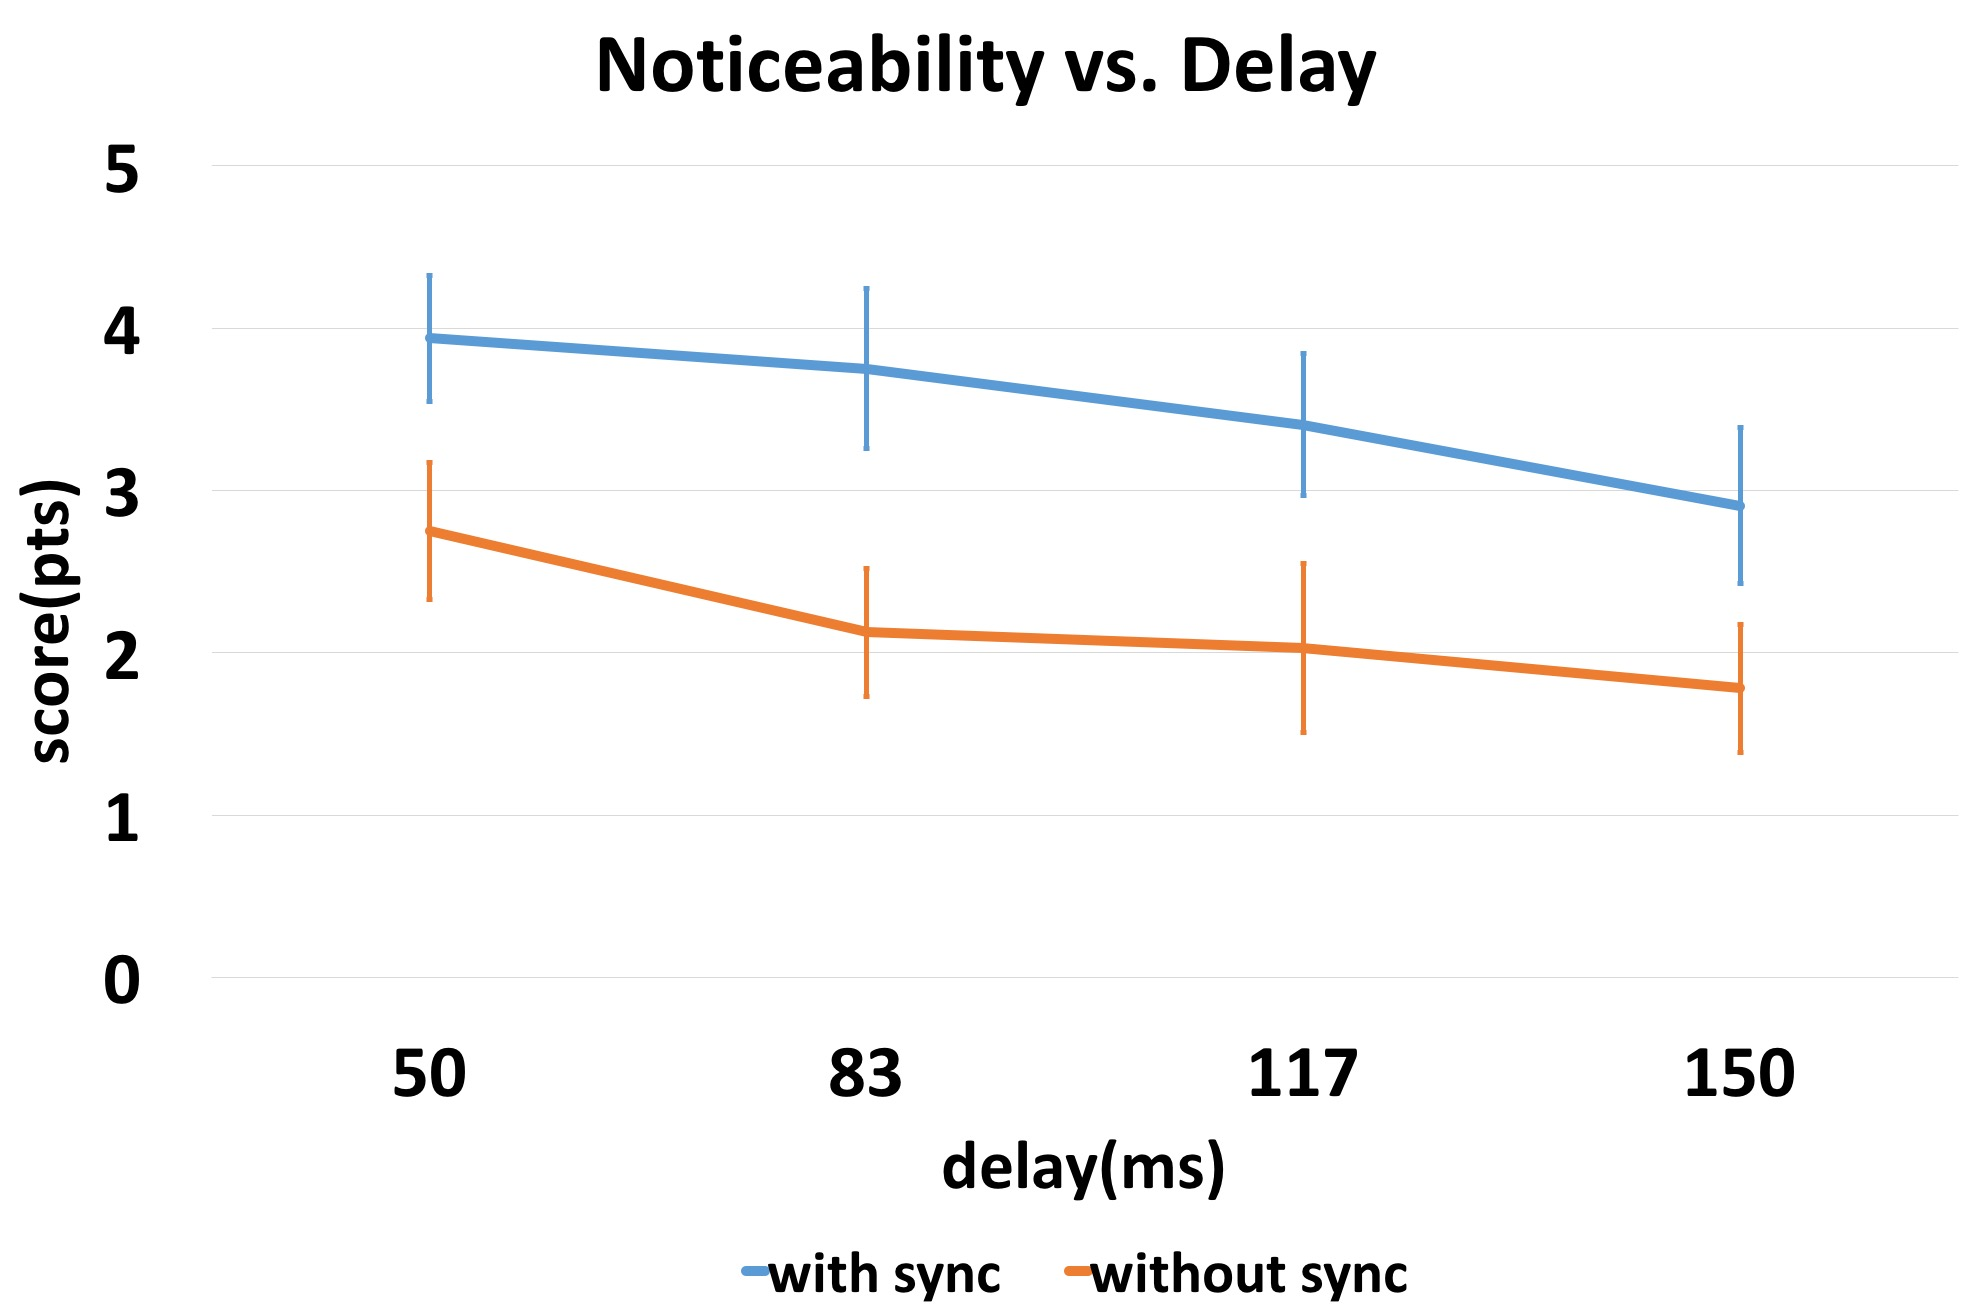
\includegraphics[width=0.9\linewidth]{figures/figure7_2.jpg}
\setlength{\abovecaptionskip}{0.5cm}
\caption{Mean Opinion Score (MOS) of noticeability versus one-way network delay.}
\label{fig:noticeability}
\end{figure}

Figure \ref{fig:noticeability} shows the results of noticeability with additional delays. The MOS value of noticeability tends to decrease as the additional delay becomes larger, except that the difference between 50 ms and 83 ms is not significant (f = xx, p < xx) with sync assistance. It shows that the sync assistance increases the threshold of noticing a network delay.

\begin{figure}[!htbp]
\centering
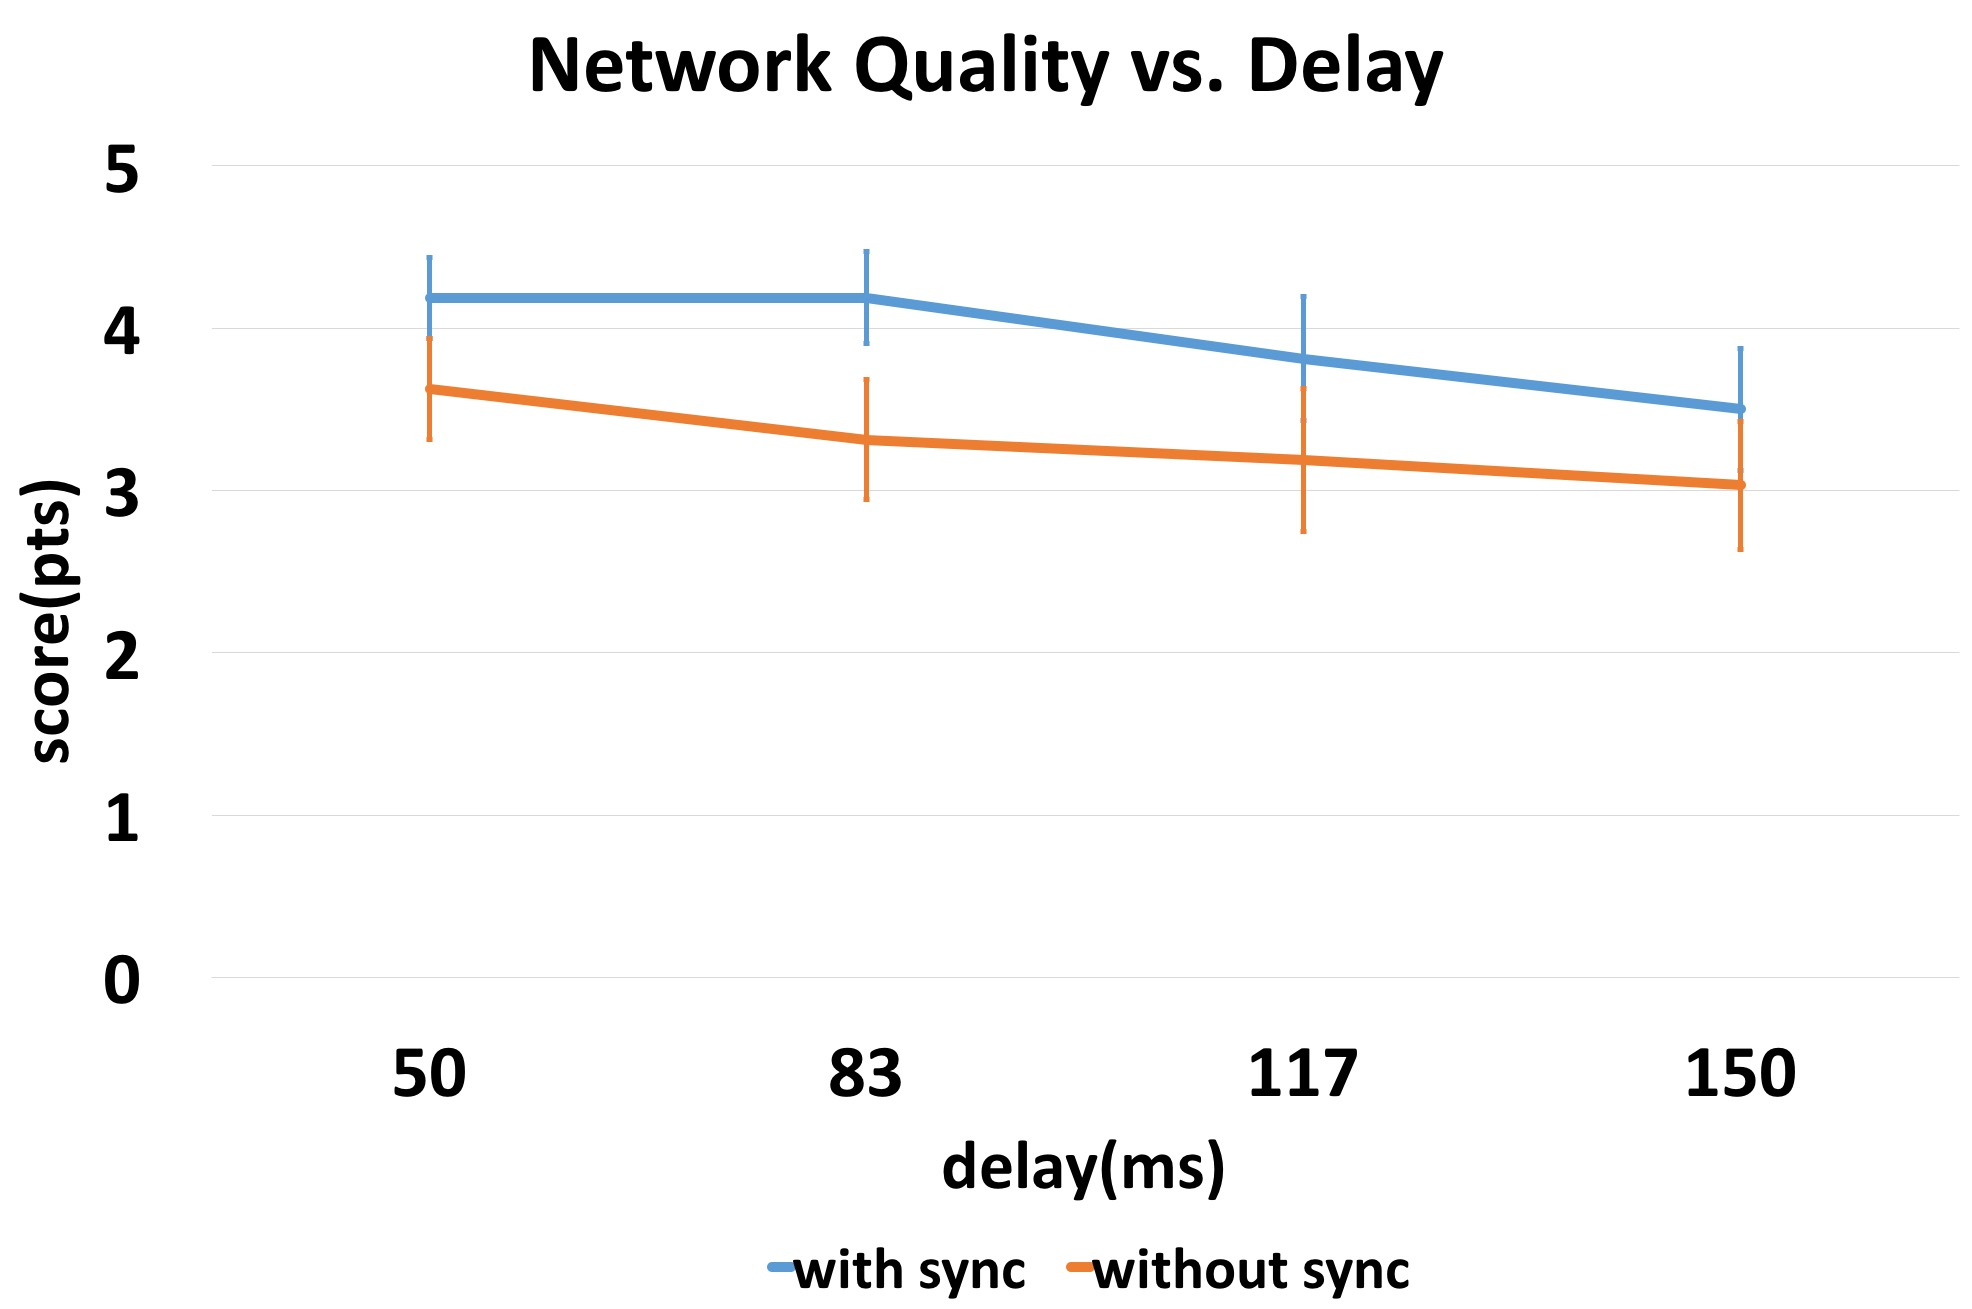
\includegraphics[width=0.9\linewidth]{figures/figure7_3.jpg}
\setlength{\abovecaptionskip}{0.5cm}
\caption{Mean Opinion Score (MOS) of network quality versus one-way network delay.}
\label{fig:overall_rating}
\end{figure}

Figure \ref{fig:overall_rating} shows the results of perceived network quality with additional delays. According to the standard of 3.5 MOS, an one-way delay of 50 ms supports a good user experience when there is no sync assistance, while 150 ms is enough with the sync assistance.

The sync assistance significantly improve the user experience in a delay-sensitive task. It can be explained by \cite{hashimoto2006influences}. In a task with synchronous actions, there should be a user who starts the task. He is the "caller". The other user just adjusts the timing of his motion to the caller' s timing. Thus, he do not perceive any network delay. In contrast, the caller experiences the round-trip delay. When there is a sync assistance, both the two users would experience an one-way delay because they actually act at the same time.

\subsection{Assessment of rendering quality}

In our system, the live 3D mesh consists of about xx triangles. The volume resolution is $256 \times 256 \times 256$ for the $2m \times 2m \times 2m$ space. The triangles are in the same size as a voxel. We record six color values in each triangle. The error of depth images is within xx mm.

\begin{figure}[!htbp]
\centering
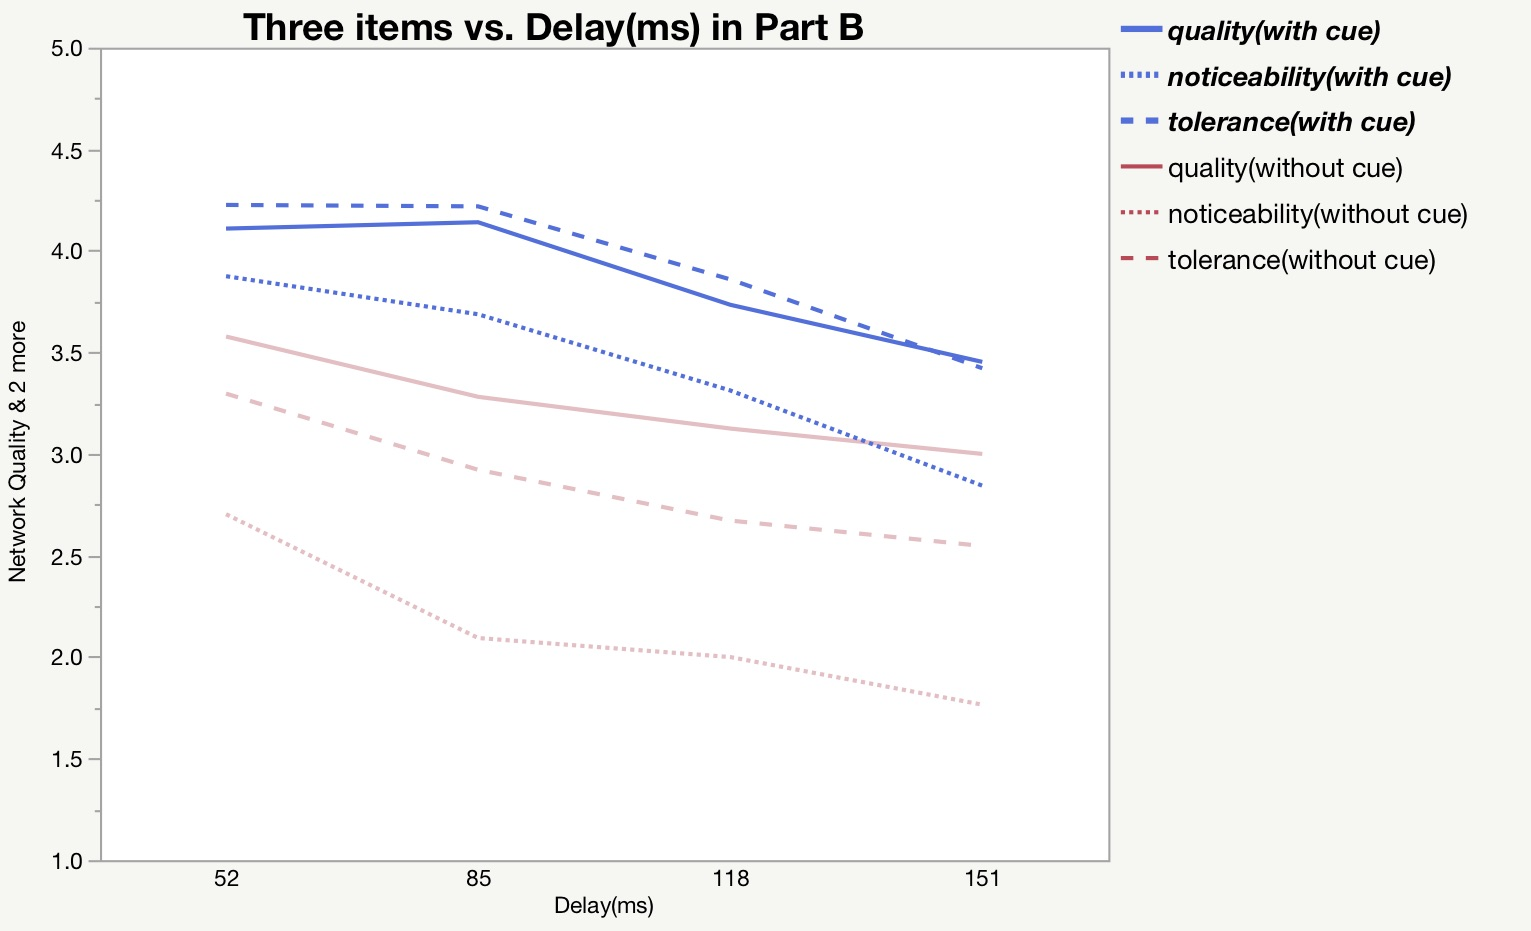
\includegraphics[width=6.9cm]{figures/figure_experiment2.jpg}
\setlength{\abovecaptionskip}{0.5cm}
\caption{(a) The percentage of participants who can accept the rendering quality. (b) Whether the rendering affects the task performance.}
\label{fig:result_quality}
\end{figure}

Figure \ref{fig:result_quality} shows the subjective feedback of the rendering quality in our system. Among the 32 users, xx users accepted the rendering quality. xx users thought that the rendering did not affect the task performance. The result shows that the rendering quality of our system is expected to be improved but somehow acceptable for related HCI researches.

\subsection{Observation and Interview}

We summarized observation notes and transcripts of interviews to reveal users' behavior in the experiment.

\subsubsection{Body language}

Through observation, we found that most participants show body language to help the communication, e.g., leaning forward to attract the partner’s attention before speaking; shrugging and spreading their hands to express confusion. In the chess game, sometimes the user need to ask his partner to remove the captured chess pieces. In this situation, he can use pointing gestures and deictic expressions (e.g., "these pieces") to refer quickly and efficiently to the task objects.

\subsubsection{Freedom to change view points}

In the chess game, some users continually change their view points to observe the chess pieces, and then aligned the pieces with the chessboard orderly. A user even told her partner to adjust his pieces, because she cannot move the chess pieces from the other side. "\emph{Please adjust this pieces, it is not aligned with the chessboard. It will affect my judgment to the game.}" A user had the the obsessiveness 

\subsubsection{Shared location and direction}

When seeing the partner through our system, the first reaction of a user may be greeting. Then, most users will try to touch the other by patting the other' s helmet or asking for handshake. These interactions are impossible in a 2D tele-communication. Though the eyes are occluded by the HMD, users tend to make eye contact by turning their head. "\emph{I intentionally looked up to my partner after I placed a piece. I wondered if he can notice it. After a few turns, I am sure that he noticed it because he also looked at me when he finished his turn.}"

\subsubsection{Confusing virtual objects with reality}

Sometimes the immersion confuses the users. Most participants ever confused the the purely virtual objects with the "real" objects. Even being informed that everything from the other was virtual, most participants unintentionally tried to move other' s chess pieces. "\emph{I know it is no use to move the black chess pieces, but the behavior is just like a kind of instinctive reaction. The pieces are just being there, which seems to be of no difference with the chess in my hand.}" This observation enlighten us to design visual cues for distinguishing the virtual objects from the reality.

\subsubsection{Sync assistance provides a psychological hint of fairness}

As we explained above, the sync assistance can halve users' perception of round-trip delay into one-way delays. However, the threshold of good experience is 50 ms without sync assistance and 150 ms with the assistance. This gap is larger than the difference between round-trip delay and one-way delay. This phenomenon can only be explained the users' mentality. The interview shows that the sync assistance provides a psychological hint of fairness in the game. "\emph{In the mode with sync assistance, I knew that the game is fair, so the network delay is tolerable for me.}"

\iffalse

\begin{figure}[!htbp]
\centering
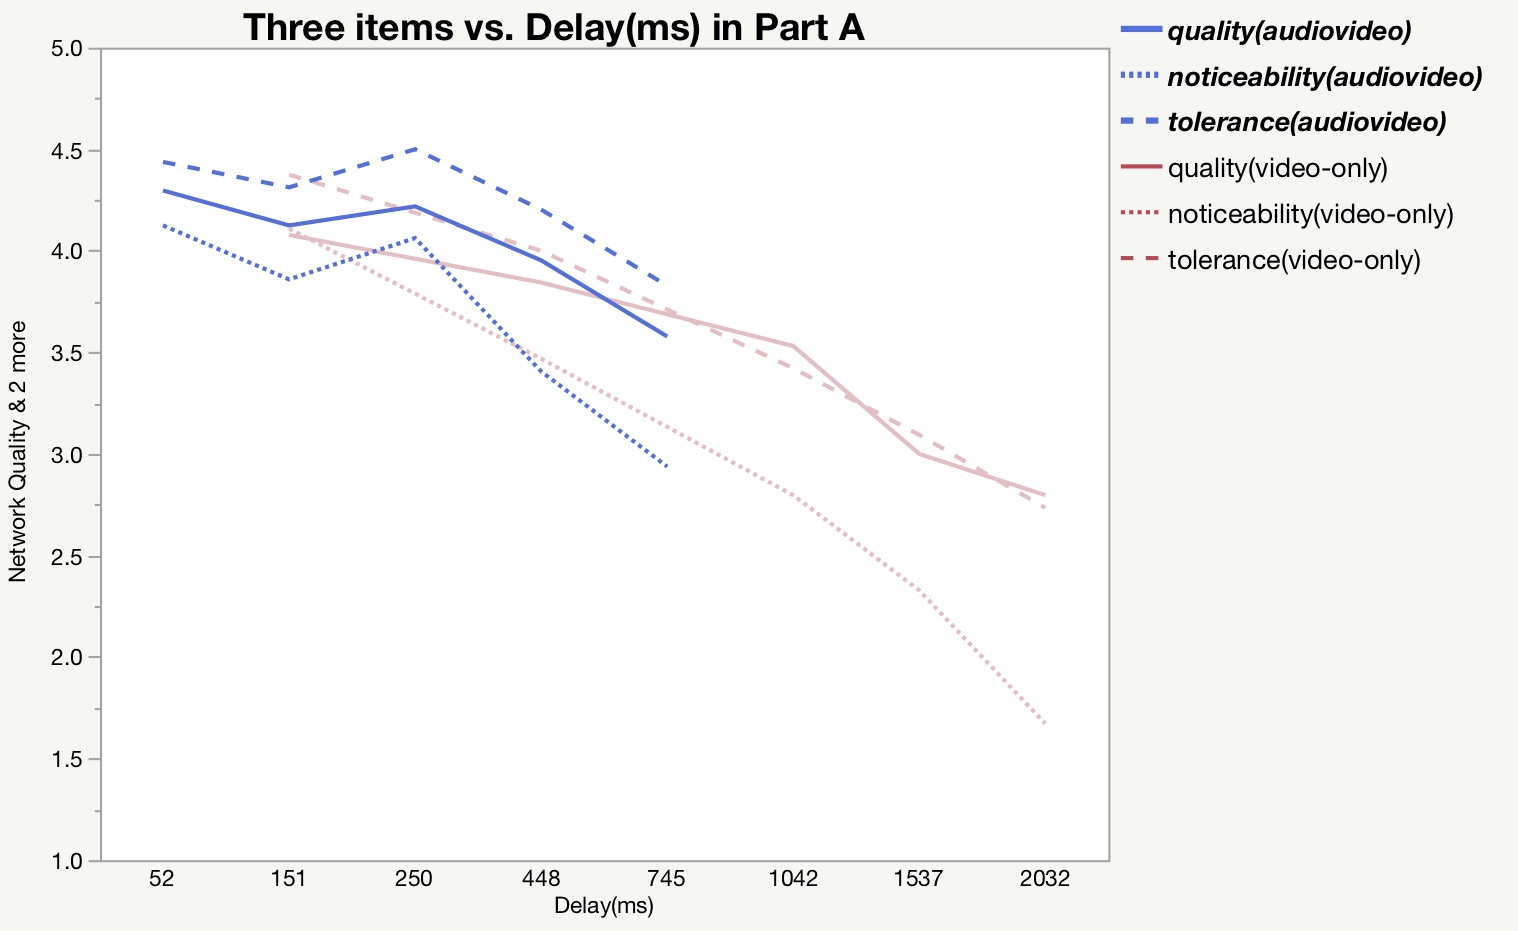
\includegraphics[width=6.5cm]{figures/figure_experiment1.jpg}
\setlength{\abovecaptionskip}{0.5cm}
\caption{Effects of delay in part A(Playing Chess).}
\label{4}
\end{figure}

Figure 7 shows the results for the three questionnaire items in part A. We tried to find out when participants started to notice the delay in audio-video and video-only tasks, so we performed a pairwise comparison between the minimum delay and other delays in each mode.

In audiovideo mode, the analysis shows that network quality is not significantly different(p = 0.1914) between 50ms and 150ms, then becomes significantly different(p = 0.042) at 450ms. For noticeability, the results follow a similar pattern. Noticeability is not significantly different(p = 0.1592) between 50ms and 150ms, then becomes significantly different(p = 0.0061) at 450ms. For annoyance, the result is still not significant(p = 0.1012) at 450ms and becomes significantly(p = 0.0058) until 750ms.

In video-only mode, the analysis shows that network quality is not significantly different(p = 0.1546) between 150ms and 450ms, then has a significant difference(p = 0.0079) at 1050ms. For noticeability(p = 0.0114) and annoyance(p = 0.0326), the result is already significant at 450ms.



Figure 8 shows the results for the three questionnaire items in part B. We used the same method as Part A to analyze delay perception in two modes.
When participants can hear synchronized audio, they gave three items significantly(p < 0.05) lower score at 117ms, but not significant(p > 0.2) at 87ms. Without the synchronized audio, noticeability score has significant(p = 0.0174) drop at 87ms, but for network quality(p = 0.0451) and annoyance(p = 0.0146), the first significant drop shows at 117ms.

Through analysis we can get the following conclusions: in 3DTI, users have more tolerance to turn-based audiovisual tasks, they still don't notice the delay at 150ms in audiovideo mode, so the recommend network delay can be increased to 200~250ms. The recommend network delays of synchronized tasks and turn-based visual-only tasks appear to rise slightly. The synchronized audio cue can help synchronization in synchronized tasks, user experience is improved with the synchronized audio.

\fi
